\documentclass[tikz,border=2mm]{standalone}
\usetikzlibrary{arrows.meta}

\begin{document}

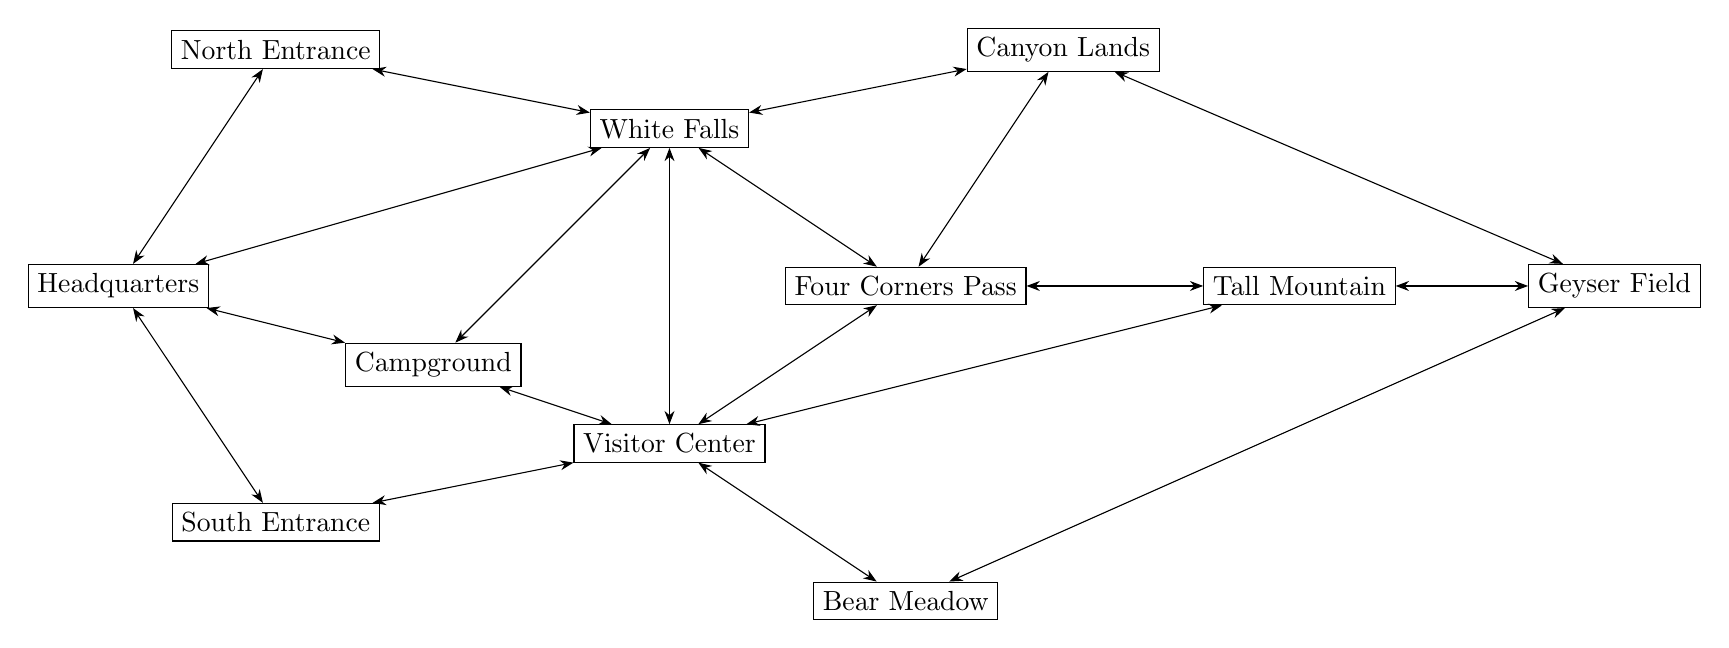
\begin{tikzpicture}[node distance=2cm and 3cm, >=Stealth]

% Define the nodes with coordinates
\node[draw, rectangle] (HQ) at (-2,0) {Headquarters};
\node[draw, rectangle] (SE) at (0,-3) {South Entrance};
\node[draw, rectangle] (NE) at (0,3) {North Entrance};
\node[draw, rectangle] (CG) at (2,-1) {Campground};
\node[draw, rectangle] (VC) at (5,-2) {Visitor Center};
\node[draw, rectangle] (WF) at (5,2) {White Falls};
\node[draw, rectangle] (FCP) at (8,0) {Four Corners Pass};
\node[draw, rectangle] (TM) at (13,0) {Tall Mountain};
\node[draw, rectangle] (CL) at (10,3) {Canyon Lands};
\node[draw, rectangle] (GF) at (17,0) {Geyser Field};
\node[draw, rectangle] (BM) at (8,-4) {Bear Meadow};

% Draw the edges without weights
\draw[<->] (HQ) -- (NE);
\draw[<->] (HQ) -- (CG);
\draw[<->] (HQ) -- (SE);
\draw[<->] (HQ) -- (WF);
\draw[<->] (SE) -- (VC);
\draw[<->] (CG) -- (VC);
\draw[<->] (CG) -- (WF);
\draw[<->] (NE) -- (WF);
\draw[<->] (WF) -- (FCP);
\draw[<->] (WF) -- (CL);
\draw[<->] (FCP) -- (CL);
\draw[<->] (FCP) -- (TM);
\draw[<->] (VC) -- (BM);
\draw[<->] (VC) -- (FCP);
\draw[<->] (VC) -- (TM);
\draw[<->] (WF) -- (VC);
\draw[<->] (CL) -- (GF);
\draw[<->] (TM) -- (GF);
\draw[<->] (BM) -- (GF);

% Highlight some edges in red
\end{tikzpicture}
\end{document}
